% Template for Cogsci submission with R Markdown

% Stuff changed from original Markdown PLOS Template
\documentclass[10pt, letterpaper]{article}

\usepackage{cogsci}


\title{Investigating children's performance on vocabulary assessments
involving object and picture stimuli in global contexts: Evidence from
Kisumu, Kenya}


\author{{\large \bf Morton Ann Gernsbacher (MAG@Macc.Wisc.Edu)} \\ Department of Psychology, 1202 W. Johnson Street \\ Madison, WI 53706 USA
  \AND {\large \bf Sharon J.~Derry (SDJ@Macc.Wisc.Edu)} \\ Department of Educational Psychology, 1025 W. Johnson Street \\ Madison, WI 53706 USA}


\begin{document}

\maketitle

\begin{abstract}
The most common assessments of early cognitive and linguistic abilities
typically involve pictures stimuli. As these assessments spread
worldwide, researchers make an implicit assumption: that children across
contexts understand pictures in the same way, at the same developmental
timepoint. What if this assumption does not hold for some or all kinds
of pictures? In the present research, a preregistered sample of 128 3-
to 7-year-olds from Kisumu, Kenya participated in a Swahili vocabulary
assessment. Using a within-subjects design, each participant completed
vocabulary trials in four formats (i.e., objects, photographs, cartoons,
black-and-white line drawings). Preregistered analyses showed that
children performed equally accurately across object, photograph, and
cartoon formats, but less accurately in the black-and-white line drawing
format. However, further exploratory analyses suggested that a subset of
black-and-white drawings drove this difference. These findings suggest
that caution is necessary in the use of picture stimuli and that
assessments involving line drawings may sometimes underestimate
children's capacities.

\textbf{Keywords:}
cognitive development, picture comprehension, cross-cultural research,
measurement
\end{abstract}

Humans possess remarkable, and potentially species-unique, capacities to
understand and use various kinds of visual media (e.g., pictures,
videos, scale models, maps). In particular, previous research shows that
high-income children growing up in Western contexts understand pictures
early in development. For example, high-income U.S. toddlers know that
pictures refer to actual objects in the world (Preissler \& Carey, 2004)
and appreciate the role of intention when interpreting pictures (Gelman
\& Ebeling, 1998). Moreover, children in these settings can learn novel
concepts from picture books and apply these concepts to actual entities
(Ganea, Ma, \& DeLoache, 2011). But how do these abilities develop?

While many cognitive scientists argue that some kind of experience with
pictures is necessary for the picture comprehension (DeLoache,
Pierroutsakos, \& Uttal, 2003; Zhu et al., 2025), it is unclear exactly
what quality and quantity of picture experience facilitates this
development. One possibility is that only minimal picture experience is
necessary for the development of full comprehension, and thus that
children across diverse environments understand pictures in similar
ways, at similar developmental timepoints. Another possibility is that
more extensive picture experience (e.g., being surrounded by picture
books, television screens, billboards, posters) is necessary for the
development of full comprehension, and thus that children living in
environments without many picture books or other visual media understand
pictures at a later timepoint than their counterparts living in
environments with an abundance of pictures. Since children growing up in
high-income, urban contexts typically all possess extensive picture
experience, cognitive scientists must work with global populations to
explore possible consistency or diversity in children's developing
capacities to understand and learn from pictures.

Moreover, the most widely used learning materials (e.g.~books, posters)
and assessments of early cognitive and linguistic abilities use picture
stimuli (Fernald, Prado, Kariger, \& Raikes, 2017). As these materials
and assessments spread across the world, researchers make the implicit
assumption that children across contexts understand pictures in the same
way, at the same developmental time point. What if this assumption does
not hold? Differences in picture comprehension can change the efficacy
of learning materials and the validity of assessments (Draper et al.,
2022; Jukes et al., 2024). Thus, it is also important to investigate
when and how children understand pictures across cultures and contexts
to determine how to appropriately translate learning materials and
assessments globally.

Indeed, there is already some evidence that picture-based assessments
may underestimate children's capacities, in some global contexts
(Callaghan et al., 2011; Walker, Walker, \& Ganea, 2013; Zhu, Kilonzo,
Engelmann, \& Gopnik, 2024). For example, preschoolers living in rural
environments in India (i.e., a village 70 kilometers from Vijayawada,
Andhra Pradesh) and Peru (i.e., a village in the rural Montaro Valley
area of the Central Highlands) performed more accurately on a false
belief task when the task was presented using objects rather than
black-and-white line drawings (Callaghan et al., 2011). Similarly, young
toddlers living in a rural village in the Kibaha-Pwani District of
Tanzania's Coast Region do not map a novel word to a novel photograph,
but succeed in mapping a novel word onto a novel object (Walker et al.,
2013). Moreover, low- to middle-income 2- to 7-year-olds in their first
month of formal schooling living in Mombasa County, Kenya (i.e., a mix
of urban and rural areas) performed significantly more accurately on an
object-based vocabulary assessment than on a cartoon-based vocabulary
assessment. In contrast, high-income urban and suburban 2- and
3-year-olds living in the San Francisco Bay Area, U.S. performed equally
accurately on object-based and cartoon-based vocabulary assessments (Zhu
et al., 2024). Furthermore, in a sample of toddlers living in urban
Kisumu, Kenya, variation in toddlers' early picture experience is
related to variation in toddlers' ability to learn from pictures(Zhu et
al., 2025). Thus, this data suggests that assessments involving pictures
may underestimate children's capacities in some global contexts.

However, more work is necessary to investigate the generalizability of
these initial findings. For example, it is unclear if these initial
findings, which were either conducted with young toddlers and
preschoolers (Callaghan et al., 2011; Walker et al., 2013; Zhu et al.,
2025) or children in their very first month of formal schooling (Zhu et
al., 2024), might generalize to older children with more formal
schooling experience, and thus likely also more picture experience.
Determining whether assessments involving pictures are appropriate for
children who have already completed some formal schooling will provide
insight into whether researchers and policy-makers need to adapt
assessments for many children in global contexts, or perhaps only the
youngest learners.

Moreover, previous cross-cultural work on children's picture
comprehension contrasted object-based tasks with only one other kind of
picture-based task (i.e., photographs, black-and-white line drawings)
(Callaghan et al., 2011; Walker et al., 2013; Zhu et al., 2024).
However, different kinds of picture stimuli may pose various advantages
and disadvantages for young children's understanding of pictures
(Pierroutsakos \& DeLoache, 2003; Simcock \& DeLoache, 2006). For
example, color photographs or cartoons may be easier for children to
understand and learn from, because they are more perceptually similar to
objects than black-and-white line drawings (Ganea et al., 2011).
However, black-and-white line drawings may be more culturally neutral
than color photographs or clipart, as the former typically depict fewer
contextually salient features (e.g., skin color). Thus, the present
experiment contrast objects with three common picture formats (i.e.,
photographs, cartoons, black-and-white line drawings), to explore
whether possible differences between object and picture stimuli hold for
multiple kinds of picture formats.

\section{Methods}\label{methods}

\subsection{Open Science Statement}\label{open-science-statement}

Preregistration, materials, deidentified data, and analysis scripts are
publicly available.

\subsection{Participants}\label{participants}

A preregistered sample of 128 Kisumu children (M = 5.39 years; range =
3.01-7.99 years; 58 girls, 70 boys; 92\% attending daycare/school; M =
2.48 years in daycare/school, range = 0-7 years in daycare/school)
participated in a Swahili vocabulary assessment. Researchers tested two
additional children whose data were excluded due to fussiness (one
child) or experimenter error (one child).

Kisumu is the third largest city in Kenya, and a relatively small metro
region containing a population of approximately one million individuals.
The majority of Kisumu households are classified as low or middle
socioeconomic status, with substantial variation in income levels and
access to basic household assets (Were et al., 2022). Thus, Kisumu
children are likely to have more variation in their picture experiences,
compared to U.S. convenience samples.

Children were recruited from a local database maintained by a local
non-profit organization, the Safe Water and AIDS Project (SWAP), and
participated in the experiment in a quiet room at the SWAP office. The
experiment was approved by a U.S. university's Committee for the
Protection of Human Subjects, as well as by the Kenya Medical Research
Institute (KEMRI), the National Commission for Science, Technology, and
Innovation (NACOSTI), and the local Kisumu County government. All
parents of child participants provided informed consent.

\subsection{Stimuli \& Procedure}\label{stimuli-procedure}

We designed a Swahili vocabulary task involving four blocks, each
presented in a different format (e.g., objects, photographs, cartoons,
black-and-white line drawings). Each block consisted of four trials,
leading to a total of sixteen trials. The order of the blocks, as well
as the order of the trials within each block, was semi-randomized across
participants.

Target words were selected from Swahili Communicative Development
Inventory (CDI) production data from two communities in Coastal Kenya
(Alcock et al., 2015). We used CDI production data, rather than
comprehension data, because there the former had more items and less
noise in the data. We found approximately 76 viable words (i.e.,
typically artifact nouns) in the Swahili CDI. We split these words into
four quartiles by age of acquisition. Each block included one target
word from each of the four quartiles, ensuring that the four blocks were
relatively similar in difficulty.

In addition to the target word, each array consisted of one near
distractor and two random distractors. Near and random distractors were
all artifacts that Kisumu children were relatively familiar with. Many
distractors were items on the Swahili CDI (Alcock et al., 2015) or used
in previous research with Kenyan preschoolers (Zhu et al., 2024).
Furthermore, local SWAP employees again confirmed that all artifacts
were familiar to Kisumu children. Similarity scores were calculated
through correlations from the THINGS database (Hebart et al., 2019).
Near distractors were conceptually similar to, and had high correlations
with, target items (average correlation = 0.82, range = 0.66-0.95).
Random distractors were less conceptually similar to, and had lower
correlations with, target items (average correlation = 0.36, range =
0.17-0.53).

\begin{CodeChunk}
\begin{figure*}[tb]

{\centering 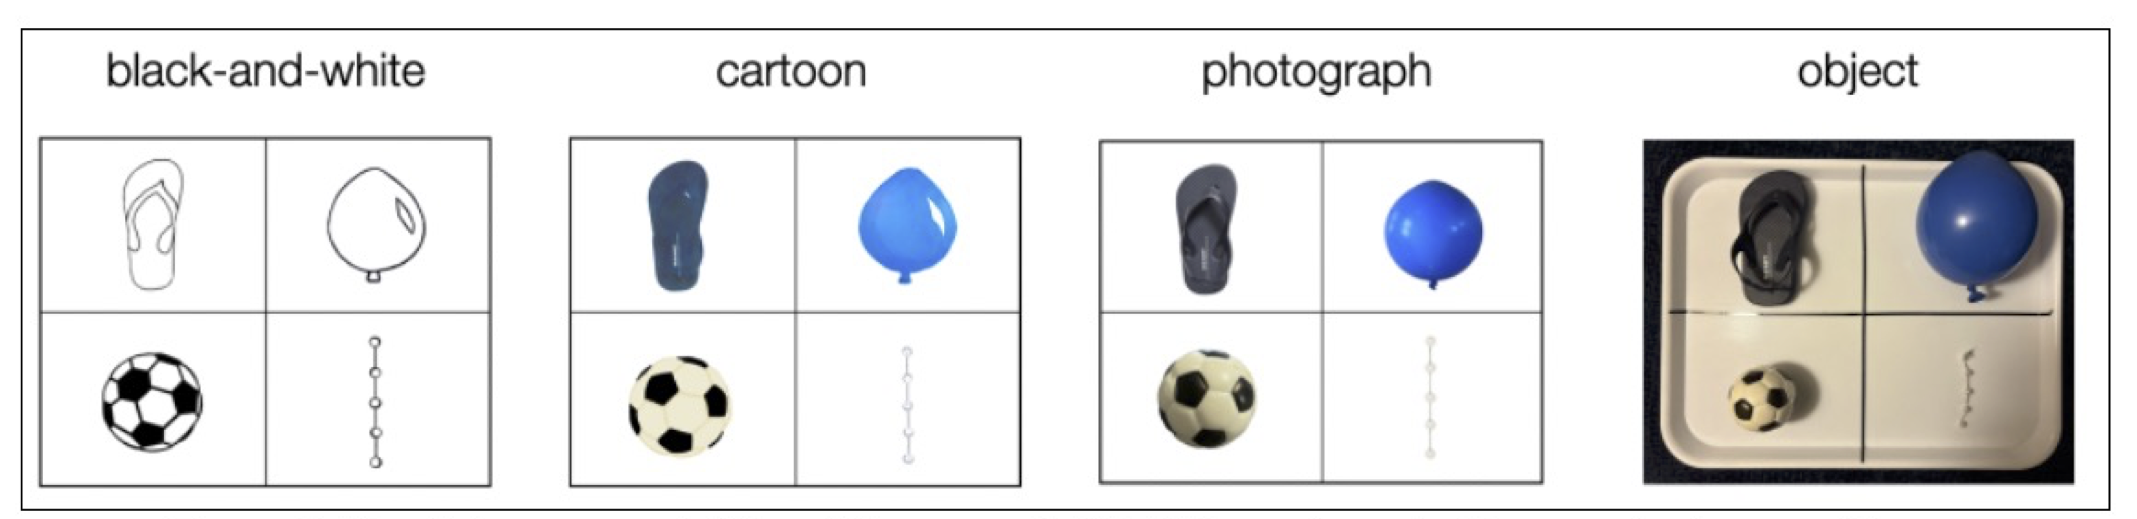
\includegraphics[width=6in]{fig1} 

}

\caption[Stimuli for a noun trial (Show me the ball / Nyoneshi mpira) across the four conditions]{Stimuli for a noun trial (Show me the ball / Nyoneshi mpira) across the four conditions.}\label{fig:figure1}
\end{figure*}
\end{CodeChunk}

Using a within-subjects design, each participant completed all sixteen
vocabulary trials. Across participants, each target word was presented
in all four formats an equal number of items. On each trial, a local
experimenter presented children with either a laminated piece of paper
depicting four objects, or a tray with four objects (see Fig. 1) and
prompted the participant to select one of the four items (e.g.,
``Nionyeshe mswaki'', meaning ``Show me a toothbrush'' in Swahili).
Within each block, the placement of the target item was counterbalanced
across trials. For a full list of target and distractor items, see Table
1.

\begin{table*}[]
\centering
\begin{tabular}{@{}ccccc@{}}
\multicolumn{1}{l}{} & \textbf{Target Item (Swahili)} & \textbf{Near Distractor} & \textbf{Random Distractor} & \textbf{Random Distractor} \\
\rowcolor[HTML]{C0C0C0}
\textbf{Set 1}       & Comb (Kichana)                 & Brush                    & Watch                      & Bracelet                   \\
\rowcolor[HTML]{C0C0C0}
\textbf{}            & Shoe (Kiatu)                   & Sock                     & Medicine                   & Telephone                  \\
\rowcolor[HTML]{C0C0C0}
\textbf{}            & Chalk (Chaki)                  & Crayon                   & String                     & Handkerchief               \\
\rowcolor[HTML]{C0C0C0}
\textbf{}            & Fork (Uma)                     & Spoon                    & Straw                      & Necklace                   \\
\textbf{Set 2}       & Cup (Kikombe)                  & Bottle                   & Soap                       & Boots                      \\
\textbf{}            & Shirt (Shati)                  & Hat                      & Eraser                     & Bucket                     \\
\textbf{}            & Scissors (Makasi)              & Knife                    & Bag                        & Bib                        \\
\textbf{}            & Button (Kifungo)               & Stone                    & Stick                      & Shovel                     \\
\rowcolor[HTML]{C0C0C0}
\textbf{Set 3}       & Book (Kitabu)                  & Paper                    & Jeans                      & Coat                       \\
\rowcolor[HTML]{C0C0C0}
\textbf{}            & Bowl (Bakuli)                  & Plate                    & Pants                      & Scarf                      \\
\rowcolor[HTML]{C0C0C0}
                     & Box (Sanduku)                  & Basket                   & Bottle Cap                 & Key                        \\
\rowcolor[HTML]{C0C0C0}
                     & Shorts (Kaptula)               & Dress                    & Clock                      & Remote Control             \\
\textbf{Set 4}       & Ball (Mpira)                   & Balloon                  & Earring                    & Sandal                     \\
                     & Toothbrush (Mswaki)            & Toothpaste               & Mirror                     & Bead                       \\
                     & Sweater (Sweta)                & Skirt                    & Glasses                    & Toilet Paper               \\
                     & Pencil (Penseli)               & Pencil Sharpener         & Towel                      & Zipper
\end{tabular}
\caption{Full list of stimuli.}
\end{table*}

\section{Results}\label{results}

\begin{CodeChunk}
\begin{figure*}[tb]

{\centering 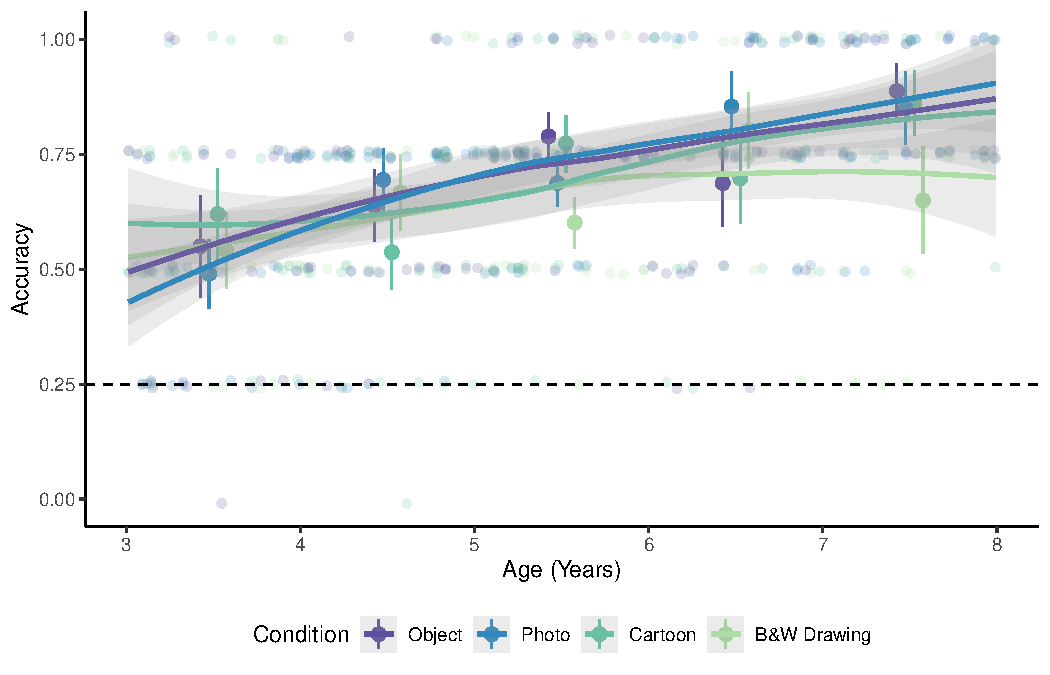
\includegraphics[width=4in]{figs/fig2-1} 

}

\caption[Proportion of accurate responses across conditions and age]{Proportion of accurate responses across conditions and age.}\label{fig:fig2}
\end{figure*}
\end{CodeChunk}

\subsection{Confirmatory Analyses}\label{confirmatory-analyses}

We fit generalized linear mixed-effects models to children's scores to
assess the factors that influenced their response accuracy. A first
preregistered mixed-effects model was fit to the response scores
(accurate/inaccurate), including fixed effects for format
(object/photograph/cartoon/black-and-white line drawing). We initially
planned to include random slopes for the effect of condition on each
child, and condition on each item. However, the model with this random
effects structure failed to converge; per lab standard operating
procedures, the reported model used the maximal random effects structure
that did converge, which included random intercepts for each child and
item. The model yielded a main effect of format, such that children were
more accurate in the object format than the black-and-white line drawing
format (\(\hat{\beta} = -0.44\), 95\% CI \([-0.78, -0.10]\),
\(z = -2.55\), \(p = .011\)). There was no difference between children's
accuracy in the object format and the photograph format
(\(\hat{\beta} = 0.00\), 95\% CI \([-0.34, 0.34]\), \(z = -0.01\),
\(p = .994\)), or in the object format and the cartoon format
(\(\hat{\beta} = -0.11\), 95\% CI \([-0.45, 0.23]\), \(z = -0.65\),
\(p = .517\)).

We also ran a second preregistered mixed-effects model including child
age as an additional variable. This second mixed-effects model was fit
to the response scores (accurate/inaccurate), including fixed effects
for format (object/photograph/cartoon/black-and-white line drawing) and
age (in years), and the interactions between format and age. We
initially planned to include random slopes for the effect of condition
on each child, and the three-way interaction between condition, age, and
item. However, the model with this random effects structure again failed
to converge, and the reported model used the maximal random effects
structure that did converge, which included random intercepts for each
child and item. The model yielded a main effect of age, such that older
children were more accurate (\(\hat{\beta} = 0.58\), 95\% CI
\([0.39, 0.77]\), \(z = 6.03\), \(p < .001\)), and a main effect of
format, such that children were more accurate in the object format than
the black-and-white line drawing format (\(\hat{\beta} = -0.48\), 95\%
CI \([-0.82, -0.14]\), \(z = -2.74\), \(p = .006\)). There was a
significant interaction between the black-and-white line drawing format
and age, such that the accuracy difference between the object and
black-and-white line drawing formats was greater for older than younger
children (\(\hat{\beta} = -0.31\), 95\% CI \([-0.56, -0.06]\),
\(z = -2.47\), \(p = .014\)). All other main effects and interactions
were not significant (all p's \textgreater{} .20).

\subsection{Exploratory Analyses}\label{exploratory-analyses}

\begin{CodeChunk}
\begin{figure*}[tb]

{\centering 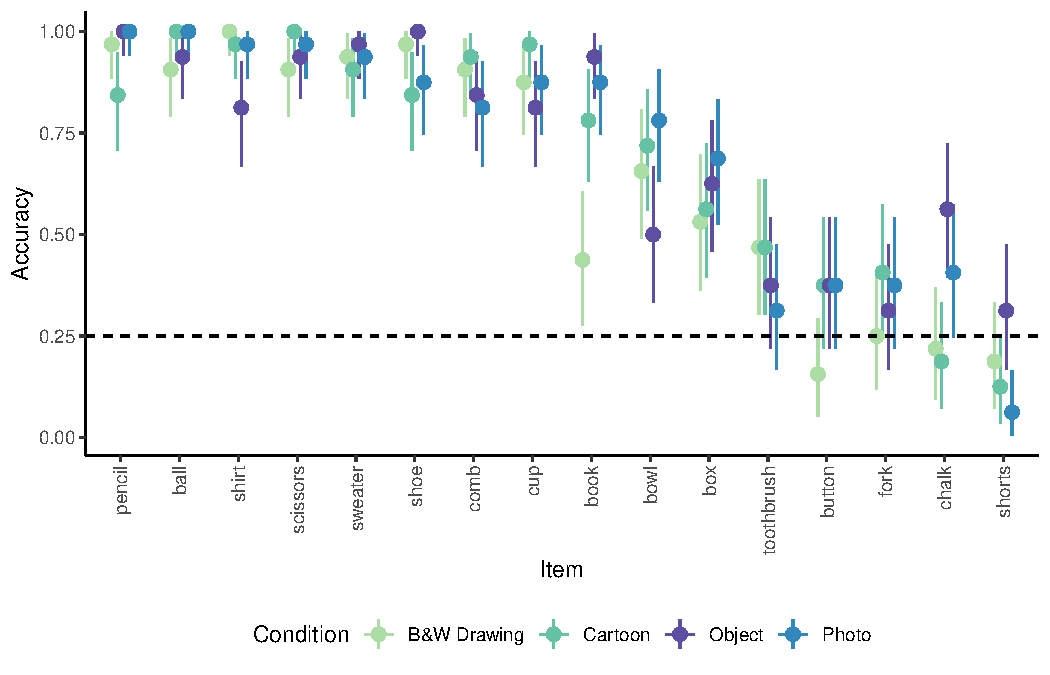
\includegraphics[width=4in]{figs/fig3-1} 

}

\caption[Response accuracy by item and condition]{Response accuracy by item and condition. Error bars are binomial 95\% confidence intervals.}\label{fig:fig3}
\end{figure*}
\end{CodeChunk}

Response accuracy was lowest in the black-and-white condition on only 6
out of 16 items, with extremely low response accuracy in the
black-and-white condition on 3 out of 16 items (i.e., ``book'',
``button'' and ``fork''; see Fig. 3). Thus, in order to explore the
model using the maximal random effects structure accounting for more
item-level variation, which did not converge in the preregistered
regressions, we also conducted exploratory Bayesian analyses. We
analyzed the data with the brms R package (Bürkner, 2017) using the
default flat priors. Each model underwent a warm- up period of 1000
iterations, followed by four sampling chains with 2000 iterations each.

A first exploratory Bayesian mixed effects model was fit to the response
scores (accurate/inaccurate), including fixed effects for format
(object/photograph/cartoon/black-and-white line drawing), and random
slopes for the effect of condition on each child, and condition on each
item. The Bayesian model converged, Gelman-Rubin statistic = 1.00. There
was no difference in performance between object and photograph formats
(papaja::apa\_print(emmeans\_bayes\_mod)\$contrasts), object and cartoon
formats, emmeans = .13, 95\% credible interval {[}-.75, 1.10{]}, or
object and black-and-white line drawing formats, emmeans = .54, 95\%
credible interval {[}-.20, 1.35{]}.

We also ran a second exploratory Bayesian mixed-effects model including
child age as an additional variable. This second mixed-effects model was
fit to the response scores (accurate/inaccurate), including fixed
effects for format (object/photograph/cartoon/black-and-white line
drawing) and age (in years), and random slopes for the effect of
condition on each child, and the three-way interaction between
condition, age, and item. This Bayesian model also converged,
Gelman-Rubin statistic = 1.00. Once again, there was no difference in
performance between object and photograph formats, emmeans = .15, 95\%
credible interval {[}-.78, .44{]}, object and cartoon formats, emmeans =
.05, 95\% credible interval {[}-.70, .74{]}, or object and
black-and-white line drawing formats, emmeans = .62, 95\% credible
interval {[}-.07, 1.31{]}.

We then ran Bayesian analyses with the same random effects structure as
the convergent preregistered models. Thus, a third exploratory Bayesian
mixed effects model was fit to response scores (accurate/inaccurate),
including a fixed effect for format
(object/photograph/cartoon/black-and-white line drawing) and random
intercepts for each child and item. The Bayesian model converged,
Gelman-Rubin statistic = 1.00. There was no difference between object
and photograph formats, emmeans = .0005, 95\% credible interval {[}-.37,
.34{]} or object and cartoon formats, emmeans = .12, 95\% credible
interval {[}-.22, .47{]}. However, there was a significant difference
between object and black-and-white line drawing formats, emmeans = .45,
95\% credible interval {[}.08, .80{]}.

A fourth exploratory Bayesian mixed effects model was fit to response
scores (accurate/inaccurate), including a fixed effect for format
(object/photograph/cartoon/black-and-white line drawing) and age (in
years), and random intercepts for each child and item. This Bayesian
model also converged, Gelman-Rubin statistic = 1.00. There was no
difference between object and photograph formats, emmeans = -.02, 95\%
credible interval {[}-.37, .34{]} or object and cartoon formats, emmeans
= .12, 95\% credible interval {[}-.25, .46{]}. However, there was a
significant difference between object and black-and-white line drawing
formats, emmeans = .48, 95\% credible interval {[}.15, .84{]}.
Consequently, the difference between children's accuracy on objects and
black-and-white line drawings is reliable, providing further support
that the random effect structure changes the significance of the effect.

\section{Discussion}\label{discussion}

The present experiment investigated whether young children in urban
Kisumu, Kenya performed equally accurately on vocabulary assessments
involving objects and three kinds of pictures (i.e., photographs,
cartoons, black-and-white line drawings). Preregistered analyses suggest
that young children in this context perform equally accurately on
vocabulary assessments involving objects, photographs, and cartoons, but
less accurately on assessments involving black-and-white line drawings.
However, further exploratory Bayesian analyses with a full random
effects model did not find significant differences in children's
response accuracy between vocabulary assessments involving objects,
photographs, cartoons, and black-and-white line drawings. These
exploratory analyses may suggest that the accuracy difference between
object-based and black-and-white line drawing-based assessments is not
consistent across items, but rather driven by specific items.
Consequently, the present experiment tentatively suggests that
assessments involving black-and-white line drawings may underestimate
the capacities of Kisumu children already attending daycare or formal
schooling, whereas cartoon- and photograph-based assessments may be
valid assessments in this population.

More data and more item diversity are required in order to conclude that
the accuracy difference between object-based and black-and-white line
drawing-based assessments is generalizable. It is possible that this
accuracy difference between objects and black-and-white line drawings
only appears for some kinds of black-and-white line drawings (e.g.,
particularly ambiguous depictions), or that the black-and-white line
drawings used in the present experiment were particularly difficult for
an idiosyncratic reason. Thus, future research should attempt to
replicate this accuracy difference between assessments involving objects
and black-and-white line drawings with a new sample of items, to better
understand whether the present finding is generalizable across items, or
driven by stimulus specificity effects.

Furthermore, what variables might account for the differences between
our present findings that Kisumu preschoolers perform equally accurately
on object-, photograph-, and cartoon-based assessments, compared to
previous findings that Mombasa preschoolers, as well as toddlers and
preschoolers in other global contexts, perform more accurately on
object- than photograph- and cartoon-based assessments (Walker et al.,
2013; Zhu et al., 2024)? One possibility is that formal schooling may
drive the discrepancy between our present findings and previous
findings. Many of the children in the present study already attend
daycares and schools, and these additional learning contexts may provide
children with more opportunities to access picture books and other kinds
of visual media, or to discuss pictures and other kinds of visual media
with teachers or peers.

Another possibility is that the children in the present study are simply
older than in previous studies. Specifically, we worked with 3- to
7-year-olds, (average age of approximately 5.5 years), whereas other
studies worked with 2-year-olds (Walker et al., 2013) and 2- to
7-year-olds, with an average age of approximately 4.5 years (Zhu et al.,
2024). Older children may have more experiences with pictures overall,
and thus perform more accurately on picture-based assessments.

A third possibility is that there is something distinct about Kisumu,
such that work from other Kenyan contexts (i.e., Mombasa County) does
not generalize to Kisumu. Indeed, Kisumu is substantially more urban
than some, though not all, previously researched global contexts, such
as rural India and Peru (Callaghan et al., 2011) and rural Tanzania
(Walker et al., 2013). In general, we caution that not all global
contexts are the same, and do not readily generalize to each other.
Instead, it is more fruitful to articulate specific variables which may
vary across and within contexts, and thus drive variation in behavior
(Bohn, Fong, Pope-Caldwell, Stengelin, \& Haun, 2024).

Thus, while the present research suggests that picture-based assessments
are indeed valid measurements in some global contexts, future work
should search for more detailed mechanistic explanations about the
development of picture comprehension. Specifically, it is still unknown
what quality and quantity of picture experience training facilitates the
development of picture comprehension.

Moreover, it is unclear whether U.S. children might perform similarly to
their Kisumu counterparts across object- and picture-based conditions.
Indeed, while previous research with toddlers and preschoolers in
Berkeley, California suggest that high-income U.S. children perform
equally accurately on vocabulary assessments involving objects and
cartoons (Zhu et al., 2024), it is unclear whether high-income U.S.
children also show no performance difference across other kinds of
picture formats. Thus, more research on picture comprehension, and
possible differences in performance across picture- and object-based
tasks, is required not only in understudied global contexts, but also
Western convenience samples.

Overall, the present findings contribute to more confidence in the
current assessments used in global contexts, particularly contexts where
children may possess highly variable amounts of picture experience.
However, much more future research is required to determine in exactly
which contexts picture-based assessments are valid or invalid.
Ultimately, this research will contribute to the development of more
inclusive and effective curricula for children worldwide, as well as
more appropriate evaluation of policies and programs to improve early
child outcomes and educational trajectories.

\section{References}\label{references}

\setlength{\parindent}{-0.1in} 
\setlength{\leftskip}{0.125in}

\noindent

\phantomsection\label{refs}
\begin{CSLReferences}{1}{0}
\bibitem[\citeproctext]{ref-alcock_developmental_2015}
Alcock, K. J., Rimba, K., Holding, P., Kitsao-Wekulo, P., Abubakar, A.,
\& Newton, C. R. J. C. (2015). Developmental inventories using
illiterate parents as informants: {Communicative} {Development}
{Inventory} ({CDI}) adaptation for two {Kenyan} languages. \emph{Journal
of Child Language}, \emph{42}(4), 763--785.
http://doi.org/\href{https://doi.org/10.1017/S0305000914000403}{10.1017/S0305000914000403}

\bibitem[\citeproctext]{ref-bohn_understanding_2024}
Bohn, M., Fong, F. T. K., Pope-Caldwell, S., Stengelin, R., \& Haun, D.
B. M. (2024). Understanding cultural variation in cognition one child at
a time. \emph{Nature Reviews Psychology}, \emph{3}(10), 641--643.
http://doi.org/\href{https://doi.org/10.1038/s44159-024-00351-8}{10.1038/s44159-024-00351-8}

\bibitem[\citeproctext]{ref-burkner_brms_2017}
Bürkner, P.-C. (2017). Brms: {An} {R} {Package} for {Bayesian}
{Multilevel} {Models} {Using} {Stan}. \emph{Journal of Statistical
Software}, \emph{80}, 1--28.
http://doi.org/\href{https://doi.org/10.18637/jss.v080.i01}{10.18637/jss.v080.i01}

\bibitem[\citeproctext]{ref-callaghan_early_2011}
Callaghan, T., Moll, H., Rakoczy, H., Warneken, F., Liszkowski, U.,
Behne, T., \& Tomasello, M. (2011). Early social cognition in three
cultural contexts. \emph{Monographs of the Society for Research in Child
Development}, \emph{76}(2), vii--viii, 1--142.
http://doi.org/\href{https://doi.org/10.1111/j.1540-5834.2011.00603.x}{10.1111/j.1540-5834.2011.00603.x}

\bibitem[\citeproctext]{ref-deloache_origins_2003}
DeLoache, J. S., Pierroutsakos, S. L., \& Uttal, D. H. (2003). The
origins of pictorial competence. \emph{Current Directions in
Psychological Science}, \emph{12}(4), 114--118.
http://doi.org/\href{https://doi.org/10.1111/1467-8721.01244}{10.1111/1467-8721.01244}

\bibitem[\citeproctext]{ref-draper_publishing_2022}
Draper, C. E., Barnett, L. M., Cook, C. J., Cuartas, J. A., Howard, S.
J., McCoy, D. C., \ldots{} Yousafzai, A. K. (2022). Publishing child
development research from around the world: {An} unfair playing field
resulting in most of the world's child population under‐represented in
research. \emph{Infant and Child Development}, No Pagination
Specified--No Pagination Specified.
http://doi.org/\href{https://doi.org/10.1002/icd.2375}{10.1002/icd.2375}

\bibitem[\citeproctext]{ref-fernald_lia_toolkit_2017}
Fernald, L., Prado, E., Kariger, P., \& Raikes, A. (2017). \emph{A
toolkit for measuring early childhood development.} Washington, D.C.:
The World Bank.

\bibitem[\citeproctext]{ref-ganea_young_2011}
Ganea, P. A., Ma, L., \& DeLoache, J. S. (2011). Young children's
learning and transfer of biological information from picture books to
real animals. \emph{Child Development}, \emph{82}(5), 1421--1433.
http://doi.org/\href{https://doi.org/10.1111/j.1467-8624.2011.01612.x}{10.1111/j.1467-8624.2011.01612.x}

\bibitem[\citeproctext]{ref-gelman_shape_1998}
Gelman, S. A., \& Ebeling, K. S. (1998). Shape and representational
status in children's early naming. \emph{Cognition}, \emph{66}(2),
B35--B47.
http://doi.org/\href{https://doi.org/10.1016/s0010-0277(98)00022-5}{10.1016/s0010-0277(98)00022-5}

\bibitem[\citeproctext]{ref-hebart_things_2019}
Hebart, M. N., Dickter, A. H., Kidder, A., Kwok, W. Y., Corriveau, A.,
Wicklin, C. V., \& Baker, C. I. (2019). {THINGS}: {A} database of 1,854
object concepts and more than 26,000 naturalistic object images.
\emph{PLOS ONE}, \emph{14}(10), e0223792.
http://doi.org/\href{https://doi.org/10.1371/journal.pone.0223792}{10.1371/journal.pone.0223792}

\bibitem[\citeproctext]{ref-jukes_principles_2024}
Jukes, M. C. H., Ahmed, I., Baker, S., Draper, C. E., Howard, S. J.,
McCoy, D. C., \ldots{} Wolf, S. (2024). Principles for {Adapting}
{Assessments} of {Executive} {Function} across {Cultural} {Contexts}.
\emph{Brain Sciences}, \emph{14}(4), 318.
http://doi.org/\href{https://doi.org/10.3390/brainsci14040318}{10.3390/brainsci14040318}

\bibitem[\citeproctext]{ref-pierroutsakos_infants_2003}
Pierroutsakos, S. L., \& DeLoache, J. S. (2003). Infants' {Manual}
{Exploration} of {Pictorial} {Objects} {Varying} in {Realism}.
\emph{Infancy}, \emph{4}(1), 141--156.
http://doi.org/\href{https://doi.org/10.1207/S15327078IN0401_7}{10.1207/S15327078IN0401\_7}

\bibitem[\citeproctext]{ref-preissler_both_2004}
Preissler, M. A., \& Carey, S. (2004). Do both pictures and words
function as symbols for 18- and 24-month-old children? \emph{Journal of
Cognition and Development}, \emph{5}(2), 185--212.
http://doi.org/\href{https://doi.org/10.1207/s15327647jcd0502_2}{10.1207/s15327647jcd0502\_2}

\bibitem[\citeproctext]{ref-simcock_get_2006}
Simcock, G., \& DeLoache, J. (2006). Get the picture? {The} effects of
iconicity on toddlers' reenactment from picture books.
\emph{Developmental Psychology}, \emph{42}(6), 1352--1357.
http://doi.org/\href{https://doi.org/10.1037/0012-1649.42.6.1352}{10.1037/0012-1649.42.6.1352}

\bibitem[\citeproctext]{ref-walker_role_2013}
Walker, C. M., Walker, L. B., \& Ganea, P. A. (2013). The role of
symbol-based experience in early learning and transfer from pictures:
{Evidence} from {Tanzania}. \emph{Developmental Psychology},
\emph{49}(7), 1315--1324.
http://doi.org/\href{https://doi.org/10.1037/a0029483}{10.1037/a0029483}

\bibitem[\citeproctext]{ref-were_comparison_2022}
Were, V., Foley, L., Turner-Moss, E., Mogo, E., Wadende, P., Musuva, R.,
\& Obonyo, C. (2022). Comparison of household socioeconomic status
classification methods and effects on risk estimation: Lessons from a
natural experimental study, {Kisumu}, {Western} {Kenya}.
\emph{International Journal for Equity in Health}, \emph{21}(1), 47.
http://doi.org/\href{https://doi.org/10.1186/s12939-022-01652-1}{10.1186/s12939-022-01652-1}

\bibitem[\citeproctext]{ref-zhu_rebecca_investigating_2024}
Zhu, R., Kilonzo, T. N., Engelmann, J., \& Gopnik, A. (2024).
Investigating the validity of assessments involving picture stimuli
across cultures and contexts: {Evidence} from young children in {Kenya}
and the {U}.{S}. \emph{PsyArXiv}.

\bibitem[\citeproctext]{ref-zhu_development_2025}
Zhu, R., Pitchik, H. O., Kilonzo, T. N., Engelmann, J., Fernald, L. C.,
\& Gopnik, A. (2025). The {Development} of {Picture} {Comprehension}
{Across} {Early} {Environments}: {Evidence} {From} {Urban} and {Rural}
{Toddlers} in {Western} {Kenya}. \emph{Developmental Science},
\emph{28}(1), e13579.
http://doi.org/\href{https://doi.org/10.1111/desc.13579}{10.1111/desc.13579}

\end{CSLReferences}

\bibliographystyle{apacite}


\end{document}
